\begin{flushright}
    \textit{Лекция 10 (от 06.10)}
\end{flushright}
\Example
Вычисление несобственных интегралов.
\begin{equation}\label{(13.9)}
    I = \int_{-\infty}^{\infty}F_{n,m}(x)dx
\end{equation}
\begin{align*}
  & F_{n,m}(x) = \frac{P_n(x)}{Q_m(x)}, \ Q_m \neq 0 \ \forall x \in \RR, \ m > n+1
\end{align*}
Пусть $R_0 \in (0, R)$,$\gamma_r = [-R;R]\cap C_R$ (см. рис. \ref{fig:13.1}).
Пусть $z_k^+$~--- нули $Q_m(z)$, причем $\Img z_k^+ > 0, \ k \in \{1, \dots,
n\}$, $R_0 = \max \sets{z_k^+}$. Пусть
\begin{align*}
  & I_R = \int_{\gamma_R}F_{n,m}(z)dz = 2 \pi i \sum_{k=1}^n\us{z_k}{\res}F_{n,m}, \ R > R_0
\end{align*}
Но
\begin{align*}
  & I_R = \int_{C_R}F_{n,m}(z)dz + \int_{-R}^RF_{n,m}(z)dz
\end{align*}
Легко заметить, что
\begin{align*}
  & \lim_{R \to \infty} \int_{C_R}F_{n,m}(z)dz = 0
\end{align*}
Значит,
\begin{equation}\label{(13.10)}
    I = \int_{-\infty}^{\infty}F_{n,m}(x)dx = 2 \pi i \sum_{k=1}^n \us{z_k}{\res} F_{n,m}
\end{equation}
\lemma
Пусть $\Phi(z)$ непрерывна на $\sets{z \mid \Img z \geq 0, \abs{z} \geq R_0 >
  0}$.
\\
Пусть $\varepsilon(R) = \max \left\{ \left| \Phi(z) \right| : z \in C_R\right\},
\ R > R_0$. Пусть $\dst \lim_{R \to \infty}R\varepsilon(R) = 0$.
\\
Тогда
\begin{align*}
  & \lim_{R \to \infty }\int_{C_R}\Phi(z)dz = 0
\end{align*}
\pr
\begin{align*}
  & \left| \int_{C_R}\Phi(z)dz \right|\leq \int_{C_R}\left| \Phi(z) \right| dz \leq \varepsilon(R) \int_{C_R}dz = \pi R \varepsilon(R) \us{R \to \infty}{\to} 0
\end{align*}
Применив лемму, докажем равенство \eqref{(13.10)}.
\begin{align*}
  & F_{n,m}(z) = \frac{z^n(1+o(1))}{z^m(1+o(1))}
\end{align*}
\begin{align*}
  & \left| F_{n,m} \right| \leq 2 \left| z \right|^{n-m} \leq 2 R^{n-m}
\end{align*}
\begin{align*}
  & R\varepsilon(R) \leq 2R^{n-m+1} \us{R \to \infty}{\to} 0
\end{align*}
Таким образом доказали формулу \eqref{(13.10)}.
\Example
Вычисление несобственных интегралов.
\begin{equation}\label{(13.11)}
    I = \int_{-\infty}^{\infty}e^{i\alpha x}F_{n,m}(x)dx
\end{equation}
\begin{align*}
  & \alpha > 0, \ F_{n,m}(x) = \frac{P_n(x)}{Q_m(x)}, \ Q_m \neq 0 \ \forall x \in \RR, \ m > n
\end{align*}
Так же, как в предыдущем примере, задаем контур и $R$. По теореме Коши о вычетах
\begin{align*}
  & I_R = \int_{\gamma_R}e^{i\alpha z}F_{n,m}(z) dz = 2 \pi i \sum_{k=1}^n\us{z_k^+}{\res}\left( e^{i\alpha z} F_{n,m}(z)\right)
\end{align*}
Покажем, что
\begin{align*}
  & const = I_R = \int_{C_R}e^{i\alpha z}F_{n,m}(z) dz + \int_{-R}^Re^{i\alpha z}F_{n,m}(z) dz \us{R \to \infty}{\to} \int_{-\infty}^\infty e^{i\alpha z}F_{n,m}(z) dz
\end{align*}
то есть
\begin{equation}\label{(13.12)}
    \lim_{R \to \infty} \int_{C_R}e^{i\alpha z}F_{n,m}(z)dx = 0 \Rightarrow I = 2 \pi i \sum_{k=1}^n \us{z_k^+}{\res}\left( e^{i \alpha z}F_{n,m}(z) \right)
\end{equation}
\lemma (Жордана)
Пусть $\Phi(z)$ непрерывна на $\left\{ z \mid \left| z \right| \geq R_0, \Img z
    \geq 0 \right\}, \ R > R_0$, $C_R$~--- семейство полуокружностей $C_R = \{z
\mid \left| z \right| = R, \Img z \geq 0\}$, $ \varepsilon(R) = \max \left\{
    \left| \Phi(z) \right| : z \in C_R \right\}$, $ \dst \lim_{R \to \infty}
\varepsilon(R) = 0$, $\alpha > 0$. Тогда
\begin{equation}\label{(13.13)}
    \lim_{R \to \infty}\int_{C_R}e^{i \alpha z}\Phi(z)dz = 0
\end{equation}
\pr
$z = x + iy \in C_R$. Значит, положим $x = R \cos \varphi$, $y = R \sin \varphi$,
$ \varphi \in [0,\pi]$. Тогда
\begin{align*}
  & e^{i \alpha z} = e^{i \alpha(x+iy)} = e^{-\alpha y + i \alpha x} = e^{-\alpha R \sin \varphi + i \alpha R \cos \varphi}
\end{align*}
\begin{align*}
  & \left| e^{i \alpha z} \right| = e^{-\alpha R \sin \varphi}
\end{align*}
\begin{align*}
  & z = R e^{i \varphi} \Rightarrow dz = R i e^{i \varphi} d \varphi
\end{align*}
\begin{align*}
  & \left| \int_{C_R}e^{i \alpha z}\Phi(z) dz \right| \leq \int_{0}^{\pi}e^{-\alpha R \sin \varphi}\varepsilon(R) R d \varphi = \varepsilon(R) R \int_{0}^{\pi}e^{-\alpha R \sin \varphi}d \varphi = 2 \varepsilon(R) R \int_{0}^{\frac{\pi}{2}}e^{-\alpha R \sin \varphi}d \varphi \leq \\
  & \leq 2 \varepsilon(R) R \int_{0}^{\frac{\pi}{2}}\exp\left( -\alpha R \frac{2 \varphi}{\pi} \right) d \varphi = \frac{2 \varepsilon(R) R \pi}{2 \alpha R}\left( 1 - e^{-\alpha R} \right) \leq \frac{\pi}{\alpha} \varepsilon(R) \us{R \to \infty}{\to} 0
\end{align*}
Здесь использовали соотношение: $\forall \varphi \in \left[ 0, \dst
    \frac{\pi}{2} \right] \ \sin \varphi \geq \dst \frac{2 \varphi}{\pi}$.
\begin{align*}
  & z = R e^{i \varphi} \Rightarrow dz = R i e^{i \varphi} d \varphi
\end{align*}
Применив лемму, докажем равенство \eqref{(13.12)}. При достаточно больших по
модулю $z$ и $m-n \geq 1$
\begin{align*}
  & \left| F_{n,m}(z) \right| \leq 2 \left| z \right|^{n-m} \leq 2 R^{n-m} \leq \frac{2}{R} \us{R \to \infty}{\to} 0
\end{align*}
\begin{align*}
  & \int_{-\infty}^\infty e^{i \alpha x}F_{n,m}(x) dx = \int_{-\infty}^\infty \cos\alpha xF_{n,m}(x) dx + i \int_{-\infty}^\infty \sin \alpha x F_{n,m}(x) dx
\end{align*}
Таким образом доказали формулу \eqref{(13.12)}.
\section{$\S 14.$ Приращение аргумента $z$ вдоль кривой}
Как известно, $z = x + iy \neq 0 \Rightarrow \Arg z = \left\{\varphi + 2 \pi k
    \mid k \in \ZZ \right\}$. Значит,
\begin{equation}\label{(14.1)}
    \cos \varphi = \frac{x}{\left| z \right|}, \ \sin \varphi = \frac{y}{\left| z \right|}
\end{equation}
\theorem
Пусть $z: [0,1] \mapsto \CC$ непрерывно дифференцируема, $\forall t \in [0,1] \
z(t)\neq 0$. Пусть $\varphi_0 = \varphi(0) \in \Arg z(0)$. Тогда существует и
единственна функция $\varphi: [0,1] \mapsto \RR$, непрерывно дифференцируемая,
$\forall t \in [0,1] \ \varphi(t) \in \Arg z(t)$, т.~е.
\begin{equation}\label{(14.2)}
    \forall t \in [0,1] \ \cos \varphi(t) = \frac{x(t)}{\left| z(t) \right|}, \ \sin \varphi(t) = \frac{y(t)}{\left| z(t) \right|}
\end{equation}
и $\varphi(0) = \varphi_0$, причем $\varphi$ явно вычисляется как
\begin{equation}\label{(14.3)}
    \varphi(t) = \varphi_0 + \int_{0}^t \frac{x(\tau)y'(\tau)-y(\tau)x'(\tau)}{x^2(\tau)+y^2(\tau)}d \tau
\end{equation}
\pr
~
\begin{itemize}
    \item Существование.
    \\
    Рассмотрим \eqref{(14.3)} и покажем, что это решение \eqref{(14.2)}.
    Определим
    \begin{equation}\label{(14.4)}
        \left\{ \begin{matrix}
                u(t) = \cos \varphi(t) \\
                v(t) = \sin \varphi(t)
            \end{matrix} \right. \Rightarrow \left\{ \begin{matrix}
                u'(t) = \varphi'(t)\sin \varphi(t) = -v(t) \varphi'(t) \\
                v'(t) = \varphi'(t)\cos \varphi(t) = u(t) \varphi'(t) 
            \end{matrix} \right.
    \end{equation}
    Определим
    \begin{equation}\label{(14.5)}
        \begin{split}
            & \left\{ \begin{matrix}
                    \tilde{u}(t) = \dst \frac{x(t)}{\left| z(t) \right|} \\
                    \tilde{v}(t) = \dst \frac{y(t)}{\left| z(t) \right|} \\
                \end{matrix} \right. \Rightarrow \\
            & \left\{ \begin{matrix}
                    \dst \frac{d}{dt} \tilde{u}(t) = \dst \frac{d}{dt}\left( \dst \frac{x}{\sqrt{x^2+y^2}} \right) = \dst \frac{x'}{\left| z \right|} - \dst \frac{2x\left( xx'+yy' \right)}{\left| z \right|^3} = -\dst \frac{y}{\left| z \right|} \cdot \dst \frac{xy'-yx'}{x^2+y^2} = - \tilde{v} \dst \frac{xy'-yx'}{x^2+y^2} \\
                    \dst \frac{d}{dt} \tilde{v}(t) = \tilde{u} \dst \frac{xy'-yx'}{x^2+y^2} \\              
                \end{matrix} \right.
        \end{split}
    \end{equation}
    Из \eqref{(14.3)} заметим, что
    \begin{align*}
      \varphi'(t) = \frac{xy'-yx'}{x^2+y^2}
    \end{align*}
    Значит, \eqref{(14.4)} и \eqref{(14.5)} задают одинаковые дифференциальные
    уравнения. Поскольку $\varphi(0) = \varphi_0$ фиксировано. то $u(0) =
    \tilde{u}(0)$, $v(0) = \tilde{v}(0)$ и по теореме единственности $u(t) =
    \tilde{u}(t)$, $v(t) = \tilde{v}(t)$, откуда следует \eqref{(14.2)}.
    \item Единственность.
    \\
    Пусть $\exists \varphi_1(t) \in \Arg z(t)$, непрерывно дифференцируемая,
    $\varphi_1(0) = \varphi_0$ (это равносильно \eqref{(14.2)}); дифференцируя,
    из \eqref{(14.4)} и \eqref{(14.5)} получаем
    \begin{align*}
      \varphi_1'(t) = \frac{xy'-yx'}{x^2+y^2}
    \end{align*}
    а значит, эта функция находится по формуле \eqref{(14.3)} и совпадает с
    $\varphi$.
\end{itemize}
\note
Формулу \eqref{(14.3)} можем записать как
\begin{equation}\label{(14.6)}
    \varphi(t) = \varphi_0 + \Img \int_{0}^t \frac{z'(\tau)}{z(\tau)}d \tau
\end{equation}
\pr
\begin{align*}
  & \frac{z'}{z} = \frac{\left( x'+iy' \right)\left( x-iy \right)}{\left( x+iy \right)\left( x-iy \right)} = \frac{x'x+y'y+i\left( xy'-x'y \right)}{x^2+y^2}
\end{align*}
\begin{align*}
  & \Img \frac{z'}{z} = \Img \frac{x'x+y'y+i\left( xy'-x'y \right)}{x^2+y^2} = \frac{xy'-x'y}{x^2+y^2}
\end{align*}
\Def
\textbf{Приращением аргумента $z$ вдоль кривой $z(t)$} на отрезке $[0,1]$
называется
\begin{equation}\label{(14.7)}
    \Delta_{[0,1]}\argt z = \varphi(1) - \varphi(0) = \Img \int_{0}^1 \frac{z'(\tau)}{z(\tau)}d \tau
\end{equation}
\begin{figure}[h!]
		\centering
		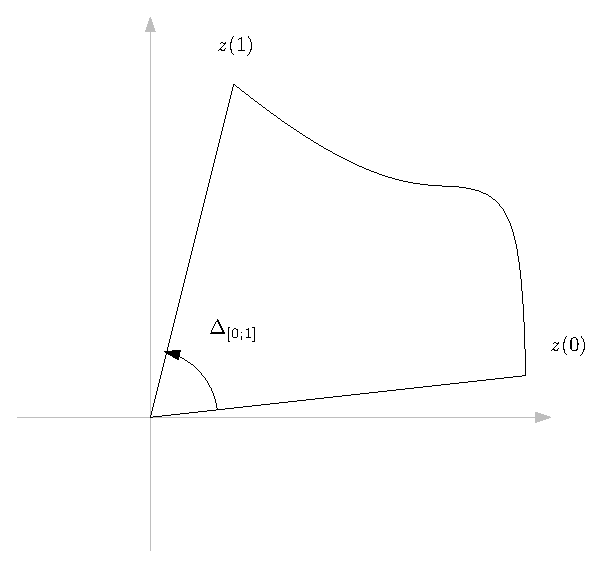
\includegraphics[scale=0.8]{deltaarg.eps}
    \caption{Приращение аргумента вдоль кривой}
		\label{fig:14.1}
\end{figure}\\
\theorem (логарифмическое свойство)
Пусть $z(t) \in C^1[0;1]$, $\forall t \in [0,1] \ z(t) \neq 0$. Пусть $z(t) =
z_1(t)z_2(t)$, $z_k(t) \in C^1[0,1]$. Тогда
\begin{equation}\label{(14.8)}
    \Delta_{[0,1]}\argt z = \Delta_{[0,1]}\argt z_1 + \Delta_{[0,1]}\argt z_2
\end{equation}
\pr
Из \eqref{(14.7)} имеем:
\begin{align*}
  & \Delta_{[0,1]} \argt z(t) = \Img \int_{0}^{1}\frac{\left( z_1(\tau)z_2(\tau) \right)'}{z_1(\tau)z_2(\tau)}d \tau =\Img \int_{0}^{1}\frac{z_1'z_2+z_1z_2'}{z_1z_2}d \tau = \Img \int_{0}^{1}\frac{z_1'}{z_1}d \tau + \Img \int_{0}^{1}\frac{z_2'}{z_2}d \tau = \\
  & = \Delta_{[0,1]} \argt z_1(t) + \Delta_{[0,1]} \argt z_2(t) 
\end{align*}
\Def
Пусть $\gamma$~--- кривая в $\CC$, заданная параметризацией $z=z(t)$, $t \in
[0;1]$, $z \in C^1[0;1]$, $0 \not \in \gamma$. Тогда \textbf{приращением
  аргумента $z$ вдоль кривой $\gamma$} называется
\begin{equation}\label{(14.9)}
    \Delta_{\gamma}\argt z = \Delta_{[0;1]}\argt z = \Img \int_{0}^1 \frac{z'(\tau)}{z(\tau)}d \tau
\end{equation}
Определение корректно, т.~к. \eqref{(14.9)} равносильно
\begin{equation}\label{(14.10)}
    \Delta_{\gamma}\argt z = \Img \int_{\gamma} \frac{dz}{z}
\end{equation}